\documentclass{article}

% packages
\usepackage{amsmath, amsthm, thmtools, amsfonts, amssymb, luacode, catchfile, tikzducks, hyperref, ifthen}
\ifcsname c@kobocompile\endcsname
	\usepackage[a5paper, total={1072pt, 1448pt}, margin=10pt, includeheadfoot]{geometry} % set page margins
\else
	\usepackage[a4paper, margin=50pt, includeheadfoot]{geometry}
\fi
\usepackage[shortlabels]{enumitem}
\usepackage[skip=3pt, indent=0pt]{parskip}

% language
\usepackage[bidi=basic, layout=tabular, provide=*]{babel}
\ifcsname c@english\endcsname
	\babelprovide[main, import]{english}
\else
	\babelprovide[main, import]{hebrew}
	\babelprovide{rl}
\fi
%\babelfont{rm}{Libertinus Serif}
\babelfont{rm}[Renderer=Harfbuzz]{Libertinus Serif}
\babelfont{sf}{Libertinus Sans}
\babelfont{tt}{Libertinus Mono}

% style
\AddToHook{cmd/section/before}{\clearpage}	% Add line break before section
\linespread{1.3}
\setcounter{secnumdepth}{0}		% Remove default number tags from sections, this won't do well with theorems
\AtBeginDocument{\setlength{\belowdisplayskip}{3pt}}
\AtBeginDocument{\setlength{\abovedisplayskip}{3pt}}
\graphicspath{ {../images/} }

% operators
\DeclareMathOperator\cis{cis}
\DeclareMathOperator\Sp{Sp}
\DeclareMathOperator\tr{tr}
\DeclareMathOperator\im{Im}
\DeclareMathOperator\re{Re}
\DeclareMathOperator\diag{diag}
\DeclareMathOperator*\lowlim{\underline{lim}}
\DeclareMathOperator*\uplim{\overline{lim}}
\DeclareMathOperator\rng{rng}
\DeclareMathOperator\Sym{Sym}
\DeclareMathOperator\Arg{Arg}
\DeclareMathOperator\Log{Log}
\DeclareMathOperator\dom{dom}
\DeclareMathOperator\supp{Supp}
\DeclareMathOperator\var{Var}
\DeclareMathOperator\cov{Cov}

% commands
%\renewcommand\qedsymbol{\textbf{מש''ל}}
%\renewcommand\qedsymbol{\fbox{\emoji{lizard}}}
\newcommand{\Aa}[0]{\mathcal{A}}
\newcommand{\Bb}[0]{\mathcal{B}}
\newcommand{\CC}[0]{\mathbb{C}}
\newcommand{\Cc}[0]{\mathcal{C}}
\newcommand{\EE}[0]{\mathbb{E}}
\newcommand{\FF}[0]{\mathbb{F}}
\newcommand{\Ff}[0]{\mathcal{F}}
\newcommand{\Ii}[0]{\mathcal{I}}
\newcommand{\Gg}[0]{\mathcal{G}}
\newcommand{\Ll}[0]{\mathcal{L}}
\newcommand{\Mm}[0]{\mathcal{M}}
\newcommand{\NN}[0]{\mathbb{N}}
\newcommand{\Nn}[0]{\mathcal{N}}
\newcommand{\PP}[0]{\mathbb{P}}
\newcommand{\Pp}[0]{\mathcal{P}}
\newcommand{\QQ}[0]{\mathbb{Q}}
\newcommand{\RR}[0]{\mathbb{R}}
\newcommand{\Rr}[0]{\mathcal{R}}
\newcommand{\Ss}[0]{\mathcal{S}}
\newcommand{\TT}[0]{\mathbb{T}}
\newcommand{\Uu}[0]{\mathcal{U}}
\newcommand{\Vv}[0]{\mathcal{V}}
\newcommand{\Ww}[0]{\mathcal{W}}
\newcommand{\ZZ}[0]{\mathbb{Z}}
\newcommand{\acts}[0]{\circlearrowright}
\newcommand{\explain}[2] {
	\begin{flalign*}
		 && \text{#2} && \text{#1}
	\end{flalign*}
}
\newcommand{\maketitleprint}[0]{ \begin{center}
	%\begin{tikzpicture}[scale=3]
	%	\duck[graduate=gray!20!black, tassel=red!70!black]
	%\end{tikzpicture}	
	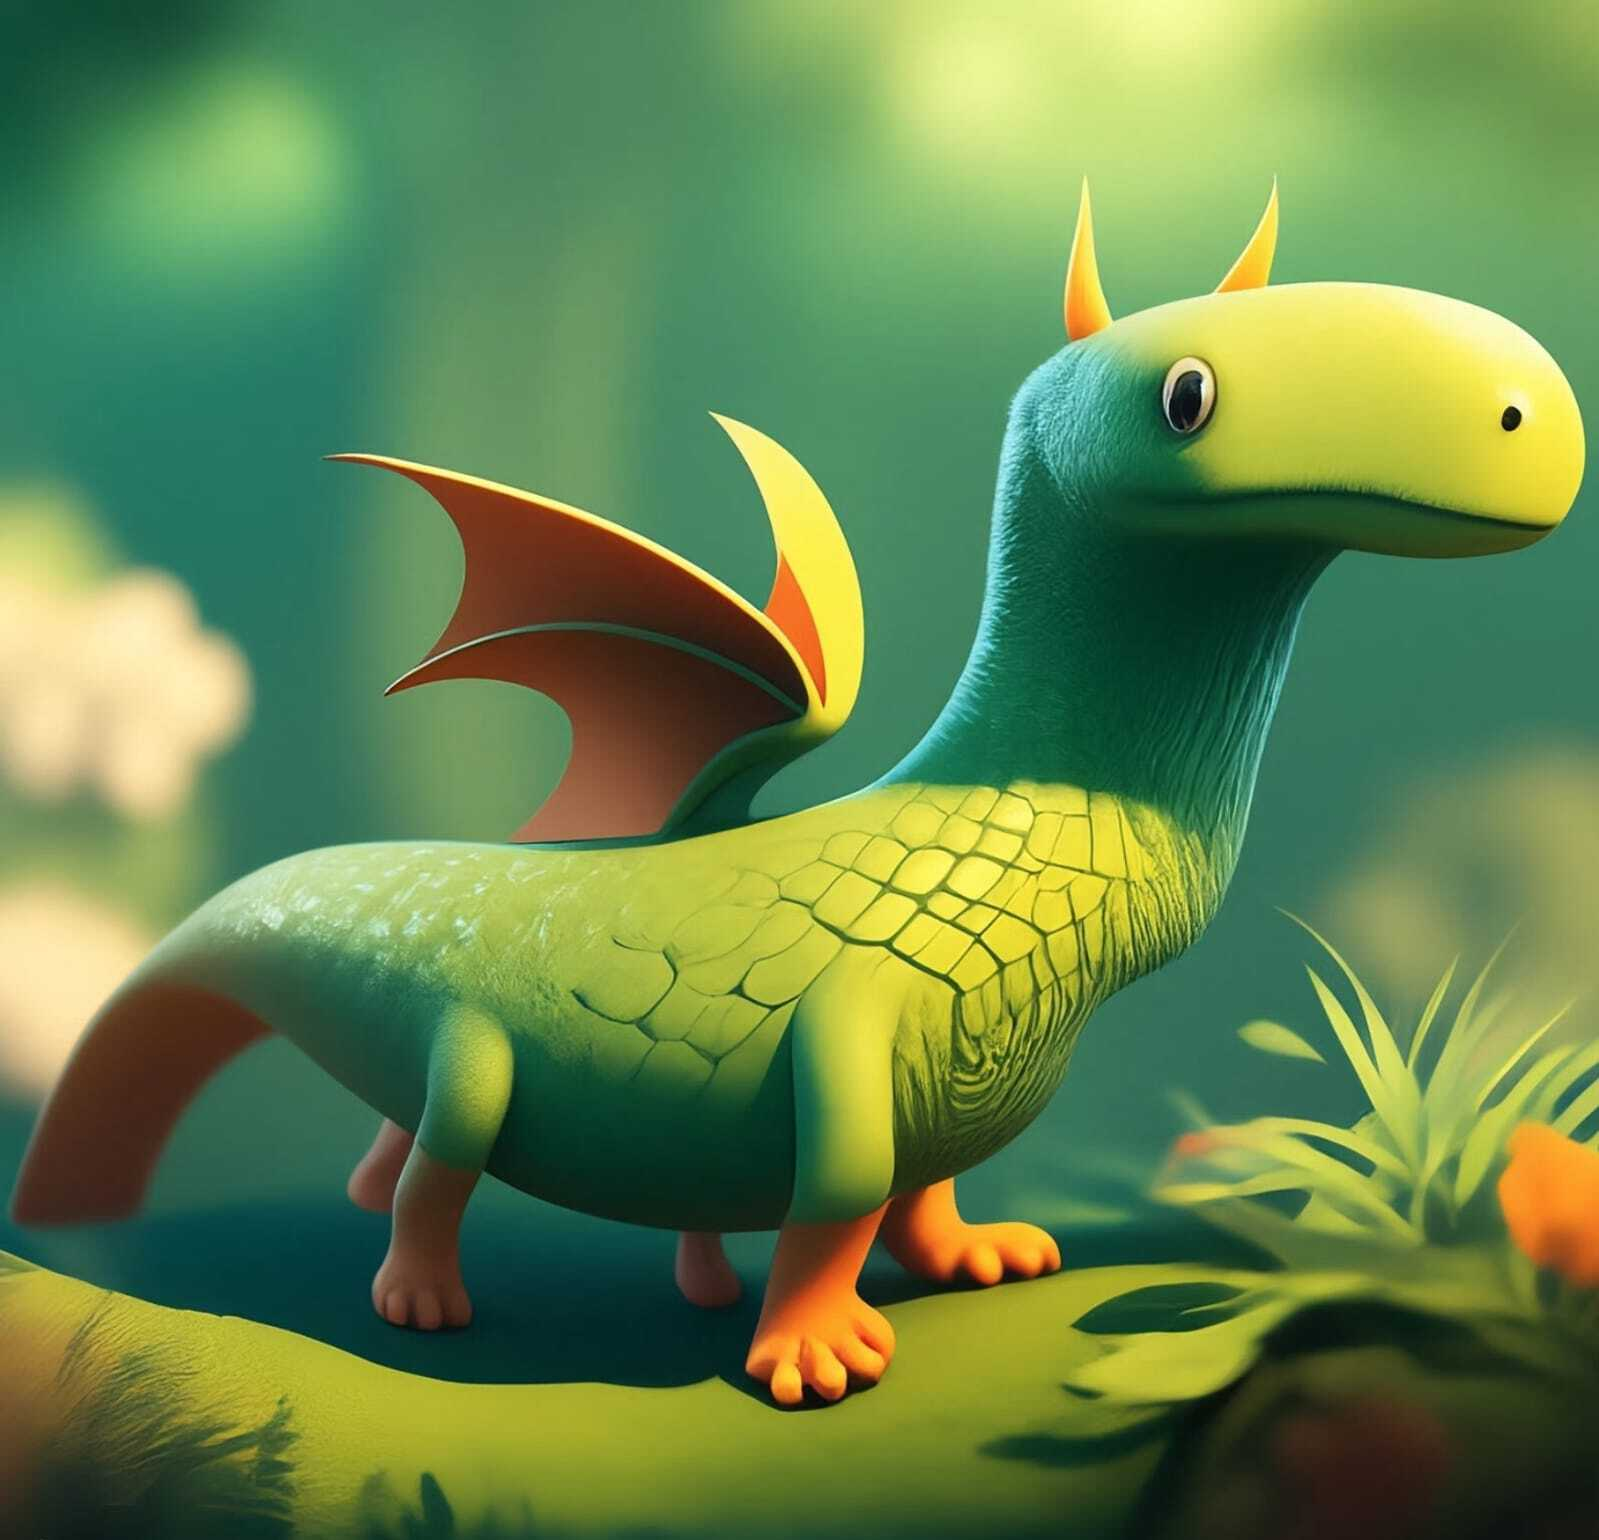
\includegraphics[width=6cm]{cover}
\end{center}
}

% theorem commands
\newtheoremstyle{c_remark}
	{}	% Space above
	{}	% Space below
	{}% Body font
	{}	% Indent amount
	{\bfseries}	% Theorem head font
	{}	% Punctuation after theorem head
	{.5em}	% Space after theorem head
	{\thmname{#1}\thmnumber{ #2}\thmnote{ \normalfont{\text{(#3)}}}}	% head content
\newtheoremstyle{c_definition}
	{3pt}	% Space above
	{3pt}	% Space below
	{}% Body font
	{}	% Indent amount
	{\bfseries}	% Theorem head font
	{}	% Punctuation after theorem head
	{.5em}	% Space after theorem head
	{\thmname{#1}\thmnumber{ #2}\thmnote{ \normalfont{\text{(#3)}}}}	% head content
\newtheoremstyle{c_plain}
	{3pt}	% Space above
	{3pt}	% Space below
	{\itshape}% Body font
	{}	% Indent amount
	{\bfseries}	% Theorem head font
	{}	% Punctuation after theorem head
	{.5em}	% Space after theorem head
	{\thmname{#1}\thmnumber{ #2}\thmnote{ \text{(#3)}}}	% head content

\ifcsname c@english\endcsname
	\theoremstyle{plain}
	\newtheorem{theorem}{Theorem}[section]
	\newtheorem{lemma}[theorem]{Lemma}
	\newtheorem{proposition}[theorem]{Proposition}
	\newtheorem*{proposition*}{Proposition}
	%\newtheorem{corollary}[theorem]{אין חלופה עברית}

	\theoremstyle{definition}
	\newtheorem{definition}[theorem]{Definition}
	\newtheorem*{definition*}{Definition}
	\newtheorem{example}{Example}[section]
	\newtheorem{exercise}{Exercise}[section]

	\theoremstyle{remark}
	\newtheorem*{remark}{Remark}
	\newtheorem*{solution}{Solution}
	\newtheorem{conclusion}[theorem]{Conclusion}
	\newtheorem{notation}[theorem]{Notation}
\else
	\theoremstyle{c_plain}
	\newtheorem{theorem}{משפט}[section]
	\newtheorem{lemma}[theorem]{למה}
	\newtheorem{proposition}[theorem]{טענה}
	\newtheorem*{proposition*}{טענה}
	%\newtheorem{corollary}[theorem]{אין חלופה עברית}

	\theoremstyle{c_definition}
	\newtheorem{definition}[theorem]{הגדרה}
	\newtheorem*{definition*}{הגדרה}
	\newtheorem{example}{דוגמה}[section]
	\newtheorem{exercise}{תרגיל}[section]

	\theoremstyle{c_remark}
	\newtheorem*{remark}{הערה}
	\newtheorem*{solution}{פתרון}
	\newtheorem{conclusion}[theorem]{מסקנה}
	\newtheorem{notation}[theorem]{סימון}
\fi

% Questions related commands
\newcounter{question}
\setcounter{question}{1}
\newcounter{sub_question}
\setcounter{sub_question}{1}

\ifcsname c@english\endcsname
	\newcommand{\question}[1][0]{
		\ifthenelse{#1 = 0}{}{\setcounter{question}{#1}}
		\section{Question \arabic{question}}
		\addtocounter{question}{1}
		\setcounter{sub_question}{1}
	}

	\newcommand{\subquestion}[1][0]{
		\ifthenelse{#1 = 0}{}{\setcounter{sub_question}{#1}}
		\subsection{Part \alph{sub_question}}
		\addtocounter{sub_question}{1}
	}
\else
	\newcommand{\question}[1][0]{
		\ifthenelse{#1 = 0}{}{\setcounter{question}{#1}}
		\section{שאלה \arabic{question}}
		\addtocounter{question}{1}
		\setcounter{sub_question}{1}
	}

	\newcommand{\subquestion}[1][0]{
		\ifthenelse{#1 = 0}{}{\setcounter{sub_question}{#1}}
		\subsection{סעיף \localecounter{letters.gershayim}{sub_question}}
		\addtocounter{sub_question}{1}
	}
\fi

% import lua and start of document
\directlua{common = require ('../common')}

\GetEnv{AUTHOR}

% headers
\author{\AUTHOR}
\date\today

\usepackage{tikz}
\DeclareMathOperator\arcsinh{arcsinh}
\title{פתרון מטלה 4 – חשבון אינפיניטסימלי 2 (80132)}

\begin{document}
\maketitle
\maketitleprint{}

\Question{}
\subsection{i.}
\begin{align*}
	\lim_{x \to 0} \frac{x^2 \cdot \sin(\displaystyle\frac{1}{x})}{\sin x}
	& = \lim_{x \to 0} \frac{x}{\sin x} \cdot x \sin \frac{1}{x} \\
	& \overset{(1)}{=} \lim_{x \to 0} \frac{x}{\sin x} \lim_{x \to 0}  x \sin \frac{1}{x} \\
	& \overset{(2)}{=} 1 \cdot \lim_{x \to \infty}  \frac{\sin x}{x} \\
	& = 1
\end{align*}
\begin{enumerate}
	\item אם הגבול קיים אז תהיה לנו הצדקה לפרק את הגבול למכפלת גבולות, נבדוק
	\item גבול ידוע, והרכבת פונקציות על $t = \frac{1}{x}$.
\end{enumerate}

\subsection{ii.}
\begin{align*}
	\lim_{x \to 0} \frac{\sin(ax)}{\sin(bx) \cdot \cos(cx)}
	& \overset{(1)}{=} \lim_{x \to 0} \frac{a \cdot \cos(ax)}{b \cdot \cos(bx) \cos(cx) - c \cdot \sin(bx) \sin(cx)} \\
	& = \frac{a \cdot 1}{b \cdot 1 - c \cdot 0} \\
	& = \frac{a}{b}
\end{align*}

\subsection{iii.}
\begin{align*}
	\lim_{x \to \infty} \frac{x + \frac{1}{2} \cos x}{x - \frac{1}{2} \sin x}
	& = \lim_{x \to \infty} \frac{1 + \frac{\frac{1}{2} \cos x}{x}}{1 - \frac{\frac{1}{2} \sin x}{x}} \\
	& = \frac{1 - 0}{1 - 0} = 1
\end{align*}

\subsection{iv.}
\begin{align*}
	\lim_{x \to 0} \frac{\tan(x) - x}{x - \sin(x)}
	& = \lim_{x \to 0} \frac{1 + \tan^2(x) - 1}{1 - \cos(x)} \\
	& = \lim_{x \to 0} \frac{\tan^2(x)}{1 - \cos(x)} \\
	& = \lim_{x \to 0} \frac{2 \tan(x) \cdot \frac{1}{\cos^2 x}}{\sin(x)} \\
	& = \lim_{x \to 0} \frac{2 \cdot \frac{1}{\cos^2 x}}{\cos(x)} \\
	& = \frac{2}{\cos^3(0)} 
	= 2
\end{align*}

\Question{}
תהי $f$ פונקציה גזירה פעמיים ב־$x_0 \in \RR$.

\Subquestion{}
נסביר מדוע קיים $\delta > 0$ כך ש־$f$ גזירה בסביבה $(x_0 - \delta, x_0 + \delta)$.

נבחן את פונקציית הנגזרת $f'(x)$, אנו יודעים כי היא גזירה בנקודה $x = x_0$ מהנתון, ולכן על־פי הגדרת הנגזרת נובע כי קיים $\delta > 0$ כך ש־$f'$ מוגדרת ורציפה ב־$(x_0 - \delta, x_0 + \delta)$.
מכאן נובע ישירות כי הפונקציה $f$ מוגדרת רציפה ובהכרח גם גזירה בסביבה זו.

\Subquestion{}
נוכיח כי הגבול קיים במובן הצר:
\[
	\lim_{h \to 0} \frac{f(x_0 + h) - 2f(x_0) + f(x_0 - h)}{h^2}
\]
\begin{proof}
	נבחן את הגדרת הנגזרת:
	\[
		f'(x_0) = \lim_{h \to 0} \frac{f(x_0 + h) - f(x_0)}{h}
	\]
	וידוע כי הנגזרת הזו היא בעצמה גזירה, דהינו:
	\begin{align*}
		f''(x_0)
		& = \lim_{h \to 0} \frac{f'(x_0 - h) - f'(x_0)}{-h} \\
		& = \lim_{h \to 0} \frac{\frac{f(x_0 + h - h) - f(x_0 - h) - f(x_0 + h) + f(x_0)}{h}}{-h} \\
		& = \lim_{h \to 0} \frac{-f(x_0 - h) - f(x_0 + h) + 2f(x_0)}{-h^2} \\
		f''(x_0) & = \lim_{h \to 0} \frac{f(x_0 - h) + f(x_0 + h) - 2f(x_0)}{h^2} \\
	\end{align*}
	וקיבלנו כי הגבול קיים ומוגדר.
\end{proof}

\Question{}
יהי $0 < \alpha \in \RR$ כלשהו.

\Subquestion{}
נוכיח כי מתקיים הגבול:
\[
	\lim_{x \to \infty} \frac{\ln x}{x}
\]
\begin{proof}
	נשים לב כי הן המונה והן המכנה שואפים לאינסוף, ונוכל להשתמש בכלל לופיטל:
	\[
		\lim_{x \to \infty} \frac{\ln x}{x}
		= \lim_{x \to \infty} \frac{1}{x}
		= 0
	\]
	ומצאנו כי הגבול מתקיים. \\*
	נשתמש במשפט ההצבה עבור $x = u^\alpha$ ונקבל:
	\[
		\lim_{u^\alpha \to \infty} \frac{\ln u^\alpha}{u^\alpha}
		= \lim_{u \to \infty} \alpha \frac{\ln u}{u^\alpha}
		= \alpha \lim_{u \to \infty} \frac{\ln u}{u^\alpha}
		= 0
	\]
	ולכן בפרט נקבל שמתקיים $\lim_{u \to \infty} \frac{\lim u}{u^\alpha} = 0$.
\end{proof}

\Subquestion{}
נוכיח שמתקיים
\[
	\lim_{x \to \infty} \frac{\ln^\alpha(x)}{x} = 0
\]
\begin{proof}
	קיבלנו כי מתקיים
	\[
		\lim_{x \to \infty} \frac{\lim x}{x^\alpha} = 0
	\]
	ונשים לב שלכל $x > e$ מתקיים $0 < \ln^\beta(x) = \beta \ln(x) < \beta \sqrt{x}$ על־פי חוקי חזקות, ולכן מכלל הסנדוויץ' נקבל
	\[
		\lim_{x \to \infty} \frac{\lim^\beta x}{x^\alpha} = 0
	\]
	נציב $\alpha = 1$ ונסמן את $\beta$ כ־$\alpha$ ונקבל גם
	\[
		\lim_{x \to \infty} \frac{\lim^\alpha x}{x} = 0
	\]
	כנדרש.
\end{proof}

\Subquestion{}
נוכיח שמתקיים הגבול $\lim_{u \to \infty} \frac{p(u)}{e^u}$ לכל פולינום $p$.
\begin{proof}
	נשתמש בגבול שקיבלנו בסעיף הקודם יחד עם ההצבה $x = e^t$ ונקבל את הגבול
	\[
		\lim_{t \to \infty} \frac{\ln^\alpha(e^t)}{e^t} = 0
		\implies
		\lim_{t \to \infty} \frac{t^\alpha}{e^t} = 0
	\]
	עתה יהי פולינום $p(x) = \sum_{n = 1}^{k} p_n x^n$. לכן נוכל לקבוע גם כי $\sum_{n = 1}^{k} p_n x^n \le \sum_{n = 1}^{k} p_{\max} x^k = k p_{\max} x^k$. \\*
	נסיק מאי־שוויון זה כי לכל $x > 0$ מתקיים $0 < p(x) < |k p_{\max}| x^k \implies 0 < \frac{p(x)}{e^x} < |k p_{\max}| \frac{x^k}{e^x}$. \\*
	ממשפט הסנדוויץ' והגבול הקודם נקבל
	\[
		\lim_{x \to \infty} \frac{p(x)}{e^x} = 0
	\]
\end{proof}

\Subquestion{}
נוכיח כי $\lim_{x \to 0^+}  x \ln x = 0$ ואף כי $\lim_{u \to 0^+} u^\alpha \ln u = 0$.
\begin{proof}
	נבחן את הביטוי בצורה $\frac{\ln x}{\frac{1}{x}}$. נבחין כי בשאיפה לאפס הן המונה והן המכנה שואפים למינוס אינסוף, ולכן נשתמש בלופיטל:
	\[
		\lim_{x \to 0^+} x \ln x 
		= \lim_{x \to 0^+} \frac{\frac{1}{x}}{\frac{-1}{x^2}} 
		= \lim_{x \to 0^+} -x
		= 0
	\]
	ומצאנו כי הגבול אכן מתקיים. \\*
	אילו נגדיר $x = u^\alpha$ ונשתמש בכלל ההצבה נקבל
	\[
		\lim_{u \to 0^+} u^\alpha \ln(u^\alpha) = 0
		\implies
		\alpha \cdot \lim_{u \to 0^+} u^\alpha \ln u = 0
		\implies
		\lim_{u \to 0^+} u^\alpha \ln u = 0
	\]
	ומצאנו כי שני הגבולות נכונים לכל $\alpha > 0$.
\end{proof}

\Question{}
נחשב את פולינומי טיילור הבאים:

\Subquestion{}
נגדיר $f(x) = x^{2024}, n = 2020, a = 0$, \\*
ולכן
\[
	P_{n, f, a}(x)
	= \sum_{i = 0}^{2020} \frac{f^{(i)}(0)}{i!} {(x - 0)}^i
	= \sum_{i = 0}^{2020} \frac{0}{i!} {(x - 0)}^i
	= 0
\]
הפולינום המתקבל הוא פולינום האפס, ולכן הוא אומנם מדויק כאשר $x = 0$, ואכן עבור $|x| < 1$ אנו יודעים כי $x^{2024}$ הוא ערך קטן ביותר, ונוכל לקרבו על־ידי $0$.

\Subquestion{}
תהי
\[
	f(x) = 3x - x^3 + x^6 - x^7 \cos x
\]
עבור $n = 5$ סביב הנקודה $a = 0$.

נבחין כי עבור $0 \le k \le 5$ מתקבל כי ${(x^7 \cos x)}^{(k)}$ הוא פונקציה המוכפלת ב־$x$, זאת אנו למדים מאינדוקציה על נגזרת מכפלת פונקציות. \\*
בהתאם ${(x^7 \cos x)}^{(k)}(0) = 0$ ולמעשה האיבר המחובר הזה לא משפיע כלל על פולינום הטיילור שעלינו לחשב. \\*
באופן דומה לסעיף הקודם נקבל כי גם $x^6$ לא משפיע על הפולינום ולכן נקבל
\[
	P_{5, f, 0}(x) = 3x - x^3
\]
גם במקרה זה הקירוב מסייע לנו להבין את גרף הפונקציה עבור $x < 1$, בו החזקות הגבוהות תורמות פחות לשינוי הפונקציה $f$.

\Question{}
יהי $n \in \NN \cup \{0\}$ ותהי $f$ פונקציה גזירה $n$ פעמים ב־$x = 0$.

\Subquestion{}
נתון ש־$g(x) = f(-x)$, נחשב את הפולינום $P_{n, g, 0}$ על־ידי הפולינום $P_{n, f, 0}$.

נבחין כי $g = f \circ h$ כאשר $h(x) = -x$, ולכן נגזרת הביטוי היא $g' = (f' \circ h) \cdot h'$, אך כמובן $h'(x) = -1$ ונקבל $g'(x) = -f'(-x)$. \\*
נוכל אם כן להוכיח באינדוקציה שמתקיים $g^{(k)}(x) = {(-1)}^k f^{(k)}(-x)$. \\*
נראה עתה כי
\[
	P_{n, g, 0}
	= \sum_{i = 0}^{n} \frac{g^{(i)}(0)}{i!} x^i
	= \sum_{i = 0}^{n} \frac{{(-1)}^i f^{(i)}(0)}{i!} x^i
	= P_{n, f \circ h, 0}
\]

\Subquestion{}
מצאנו בהרצאה כי עבור $f(x) = \frac{1}{1 - x}$ מתקיים
\[
	P_{n, f, 0} = \sum_{i = 0}^{n} x^i
\]
נשתמש בפולינום זה כדי למצוא את $P_{n, g, 0}$ כאשר $g(x) = \frac{1}{1 + x}$.

נשים לב כי מתקיים $g = f \circ h$ עבור $h$ מהסעיף הקודם ולכן נובע:
\[
	P_{n, g, 0}
	= P_{n, f \circ h, 0}
	= \sum_{i = 0}^{n} {(-1)}^i x^i
\]

\Subquestion{}
נגדיר עתה $h(x) = \ln(1 + x)$ ונחשב את פולינום טיילור שלה סביב $0$.

נבחין כי $h'(x) = \frac{1}{1 + x} = g(x)$ מהסעיף הקודם. \\*
בהתאם נראה כי $h^{(k)}(x) = h^{(k - 1)}(x)$ וכי $h(0) = \ln 1 = 0$ ונסיק
\[
	P_{n, h, 0}
	= \sum_{i = 0}^{n} \frac{{(-1)}^i x^{i + 1}}{i + 1}
\]

\Question{}
יהי $m \in \NN$ ותהי פונקציה $f$ גזירה אינסוף פעמים בנקודה $a = 0$.
לכל $k \in \NN \cup \{0\}$, נסמן $P_k = P_{k, f, 0}$.

\Subquestion{}
\subsubsection{i.}
נוכיח שהקבוצה $A = \Sp\{ f^{(k)}(x^m)h(x) \mid k \in \NN \cup \{0\}, h \in \RR[x]\}$ סגורה תחת פעולת הגזירה ואף כי הפונקציה $g$ המוגדרת על־ידי $g(x) = f(x^m)$ גזירה אינסוף פעמים ב־$0$.
\begin{proof}
	יהי $k \in \NN \cup \{0\}$ ו־$h \in \RR[x]$, לכן $f^{(k)}(x^m)h(x) \in A$.
	נגזור את הביטוי ונקבל
	\begin{align*}
		(f^{(k)}(x^m)h(x))'
		& = (f^{(k)}(x^m))'h(x) + f^{(k)}(x^m)h'(x) \\
		& = f^{(k + 1)}(x^m)h(x) \cdot (x^m)' + f^{(k)}(x^m)h'(x) \\
		& = f^{(k + 1)}(x^m)h(x) \cdot mx^{m - 1} + f^{(k)}(x^m)h'(x) \\
	\end{align*}
	אנו יודעים כי מרחב הפולינומים סגור לכפל ולגזירה, ולכן נובע כי $mx^{m - 1}h(x), h'(x) \in \RR[x]$. \\*
	מכאן נסיק ישירות כי $(f^{(k)}(x^m)h(x))' \in A$.

	עתה נבחין כי עבור $h(x) = 1$ נקבל $g(x) = f(x^m) \cdot 1 \in A$, ומצאנו כי הקבוצה סגורה לגזירה, ולכן נוכל להוכיח באינדוקציה כי $\forall k \in \NN: g^{(k)} \in A$.
\end{proof}

\subsubsection{ii.}
יהי $n \in \NN \cup \{0\}$, נוכיח ש־$Q(x) = P_n(x^m)$ שקול ל־$P_{nm, g, 0}$.
\begin{proof}
	נבחן את הגבול
	\[
		\lim_{x \to 0} \frac{g(x) - P_n(x^m)}{x^{mn}}
		= \lim_{x \to 0} \frac{f(x^m) - P_n(x^m)}{x^{mn}}
	\]
	נשתמש בכלל ההצבה עבור $t = x^m$ ונקבל
	\[
		\lim_{x \to 0} \frac{f(x^m) - P_n(x^m)}{x^{mn}}
		= \lim_{t \to 0} \frac{f(t) - P_n(t)}{t^n}
		= 0
	\]
	על־פי המשפט לקירובי טיילור בנקודה. לכן נובע כי גם
	\[
		\lim_{x \to 0} \frac{g(x) - P_n(x^m)}{x^{mn}}
		= 0
	\]
	ולכן על־פי ההגדרה $P_n(x^m)$ הוא קירוב טיילור מסדר $nm$ עבור $g$ ב־$x = 0$.
\end{proof}

\Subquestion{}
נחשב את פולינום טיילור של $g(x) = \frac{1}{1 + x^m}$ סביב אפס.

נבחין כי עבור $f(x) = \frac{1}{1 + x}$ מתקבל ש־$g(x) = f(x^m)$. \\*
בסעיף 5א' מצאנו גם כי
\[
	P_n(x) = \sum_{i = 0}^{n} \frac{{(-1)}^i x^{i + 1}}{i + 1}
\]
ולכן מהסעיף הקודם נובע
\[
	P_{nm, g, 0} = P_n(x^m)
	= \sum_{i = 0}^{n} \frac{{(-1)}^i x^{m(i + 1)}}{i + 1}
\]

\Subquestion{}
נחשב את פולינום טיילור מסדר $2n + 1$ של $h(x) = \arctan x$ סביב $0$.

נבחין כי $h'(x) = \frac{1}{x^2 + 1}$ על־פי המטלות הקודמות. לכן נסיק מהסעיף הקודם כי
\[
	P_{2n, h', 0}(x)
	= \sum_{i = 0}^{n} \frac{{(-1)}^i x^{2(i + 1)}}{i + 1}
\]
נשתמש בכלל שמצאנו בכיתה עבור פולינום טיילור ונגזרת:
\[
	(P_{2n + 1, h, 0}(x))'
	= P_{2n, h', 0}(x)
	= \sum_{i = 0}^{n} \frac{{(-1)}^i x^{2(i + 1)}}{i + 1}
\]
ונשים לב שמקרה זה מתקיים כאשר:
\[
	P_{2n + 1, h, 0}(x)
	= \sum_{i = 0}^{n} \frac{{(-1)}^i x^{2i + 1}}{2n + 1}
\]

\end{document}
